%%
%% CSE 8673 (Machine Learning), Fall 2026, Mississippi State University
%% Term paper: 8-page conference draft, double column (ACM sigconf).
%% Overleaf project name: AditPatel_BiomedicalML_CSE_8673
%%
%% Phase 0 set the title and abstract. Phase 1 added the literature survey
%% and the paper list in literature_list.csv. Phase 2 reorganized the paper
%% to follow the course template (TERM_PAPER_TEMPLATE_DATAPOINTS): research
%% challenges, proposed methodology, experimental methodology, planned
%% results, the six-week plan, and the two required sections at the end.
%% The Phase 1 version is in Overleaf's history.
%%
%% Compile with pdfLaTeX + BibTeX (Overleaf default).
%% "nonacm" removes the ACM copyright block and reference-format box,
%% since this is a course paper and not an ACM submission.
%%
\documentclass[sigconf,nonacm]{acmart}

\AtBeginDocument{%
  \providecommand\BibTeX{{%
    Bib\TeX}}}

\usepackage{amsmath}
\usepackage{booktabs}
\usepackage[edges]{forest}
\usepackage{tikz}
\usetikzlibrary{arrows.meta,fit}
\usepackage{tabularx}

%% Left-aligned table columns. P{width} has a fixed width and L stretches.
\newcolumntype{P}[1]{>{\raggedright\arraybackslash}p{#1}}
\newcolumntype{L}{>{\raggedright\arraybackslash}X}

%% Let a column end short instead of stretching the space between blocks.
\raggedbottom

%% Page numbers, so page counts are easy to check.
\settopmatter{printfolios=true}

\begin{document}

\title{Group-Robust Shift-Aware Temperature Scaling for Adapted Medical
  Foundation Models Under Image Corruption}

\author{Adit Patel}
\affiliation{%
  \institution{Mississippi State University}
  \department{Department of Computer Science and Engineering}
  \city{Mississippi State}
  \state{Mississippi}
  \country{USA}}
  \email{adp543@msstate.edu}

\renewcommand{\shortauthors}{Patel}

\begin{abstract}
Medical foundation models are usually adapted to a new task by linear
probing or LoRA and then calibrated with temperature scaling on clean
validation data. Test images are often degraded by noise, blur, or changes
in lighting, and a calibrator fit on clean data can become overconfident
under this kind of shift, possibly more for some patient groups than for
others. Shift-aware calibrators only target average calibration, and
group-aware calibrators assume that test data look like calibration data. I
propose Group-Robust Shift-Aware Temperature Scaling (GR-SATS), a post-hoc
calibrator that sets a per-image temperature from a standardized
nearest-neighbor shift score and fits its two parameters for the worst-off
patient group. The fit is convex and needs group labels only while fitting.
I will evaluate it on HAM10000 with sex and age groups and on Fitzpatrick17k
with skin-type groups, using DINOv2 and BiomedCLIP backbones adapted by
linear probing and LoRA, under MedMNIST-C corruptions at five severity
levels. Each calibrator is tested on corruption families it did not see
during fitting and compared with temperature scaling variants, density-aware
calibration, atypicality-aware recalibration, and cluster-wise and group-wise
temperature scaling, with worst-group negative log-likelihood and Brier score
as the main metrics. The expected contribution is, as far as I know, the
first worst-group, shift-aware post-hoc calibrator for medical imaging, along
with a measurement of how subgroup calibration degrades under corruption for
different adaptation strategies.
\end{abstract}

\begin{CCSXML}
<ccs2012>
 <concept>
  <concept_id>10010147.10010257</concept_id>
  <concept_desc>Computing methodologies~Machine learning</concept_desc>
  <concept_significance>500</concept_significance>
 </concept>
 <concept>
  <concept_id>10010405.10010444</concept_id>
  <concept_desc>Applied computing~Life and medical sciences</concept_desc>
  <concept_significance>300</concept_significance>
 </concept>
</ccs2012>
\end{CCSXML}

\ccsdesc[500]{Computing methodologies~Machine learning}
\ccsdesc[300]{Applied computing~Life and medical sciences}

\keywords{calibration, temperature scaling, distribution shift, image
  corruption, fairness, subgroup robustness, medical foundation models}

\maketitle

%% =========================================================
\section{Introduction}
\label{sec:intro}

Foundation models pretrained on large image collections are now a common starting point for medical image classification \cite{moor2023generalist,oquab2024dinov2,zhang2025biomedclip}. They are usually adapted to the task before use, either by training a linear head on frozen features, called linear probing (LP), or by fine-tuning a small set of added low-rank weights with LoRA \cite{hu2022lora,jin2024fairmedfm}. In dermatology, an adapted model might estimate the probability that a lesion is malignant, and a clinician might use that number to decide whether to biopsy. This only works if the probabilities are calibrated, so that about 20\% of the lesions given a 20\% risk are actually malignant \cite{guo2017calibration}. Calibrated risks help patients, and they help clinicians decide when to trust or overrule the model.

The problem is that calibration is usually checked on clean validation images, while real images vary in quality. Clinical photos can be blurry, compressed, or badly lit, and dermoscopy images can have black corners from the dermatoscope or text from camera overlays \cite{disalvo2024medmnistc}. Calibration gets worse as images move away from the training distribution \cite{ovadia2019trust}, and post-hoc calibrators fit on clean data become overconfident under this kind of shift \cite{tomani2021posthoc}. Calibration also differs between patient groups. Dominique et al.\ found that leading skin cancer models overestimated risk and were miscalibrated across sex, skin tone, and age groups on new datasets \cite{dominique2025calibration}, and Groh et al.\ found that a skin condition classifier was most accurate on skin types similar to the ones it was trained on \cite{groh2021fitzpatrick}. The groups most at risk also tend to be the smallest. In the cleaned Fitzpatrick17k \cite{abhishek2025quality}, skin types V and VI make up 11\% of the images with a known skin type, and its validation and test sets together hold only 32 cancers from these two types. If calibration breaks under corruption, these patients are the ones most likely to get overconfident risk estimates, and the small numbers make the failure hard to see.

Several lines of work cover parts of this problem. Temperature scaling (TS) fits a single temperature on clean validation data \cite{guo2017calibration}. Shift-aware calibrators are fit on perturbed validation data \cite{tomani2021posthoc}, learn temperatures from several domains \cite{yu2022multidomain}, or let the temperature depend on how far an input is from the training data, as density-aware calibration (DAC) does with nearest-neighbor distances \cite{tomani2023dac} and atypicality-aware recalibration (AAR) does with class-conditional Gaussians \cite{yuksekgonul2023atypicality}. On the fairness side, multicalibration and FairCal calibrate within groups or clusters \cite{hebertjohnson2018multicalibration,salvador2022faircal}, GroupDRO and Cluster-Focal train for the worst-off group \cite{sagawa2020groupdro,shui2023clusterfocal}, and MEDFAIR and FairMedFM benchmark group gaps of medical models \cite{zong2023medfair,jin2024fairmedfm}. MedMNIST-C supplies realistic corruptions for medical images \cite{disalvo2024medmnistc}.

Although shift-aware calibrators keep average calibration under shift, none of them targets the worst-off patients, and group-aware calibrators assume that test images look like the calibration images. This matters because fairness measured in distribution often does not hold out of distribution \cite{schrouff2022diagnosing,yang2024limits}. FairMedFM reports gaps in expected calibration error (ECE) between groups only on clean test images, MEDFAIR's shift tests use chest X-ray and brain MRI dataset pairs and not graded corruption, and MedMNIST-C reports no calibration metrics at all. As far as I know, no published work in medical imaging has measured how subgroup calibration changes with corruption severity, or how that depends on the adaptation strategy. So there is a need for a post-hoc calibrator that is shift-aware and also protects the worst-off group, and for a careful measurement of when clean-fit calibration stops working.

I propose Group-Robust Shift-Aware Temperature Scaling (GR-SATS). Each image gets a shift score, the standardized log distance from its features to its nearest clean training images. The inverse temperature is a linear function of this score, and its two parameters are fit to minimize the negative log-likelihood (NLL) of the worst-off group, in the spirit of GroupDRO. This should help because corrupted images and images from rare groups both sit farther from the training data, so a temperature that rises with the shift score can lower confidence where predictions are least reliable, and the worst-group fit decides how fast it rises for the group that needs it most. Group labels are only needed while fitting, so at test time the calibrator works on any adapted model without retraining. Because the inverse temperature is linear in the parameters, the worst-group fit is a convex problem that can be solved exactly. I will test GR-SATS on two dermatology datasets with two backbones and two adaptation strategies, always on corruption families that the calibrator did not see during fitting. The main contributions of this work are summarized as follows.

\begin{itemize}
  \item \textbf{A worst-group, shift-aware calibrator.} GR-SATS has a convex two-parameter fit and needs no group labels at test time. I also test a variant with a shift-dependent bias for groups whose risks are off in one direction, and a worst-group version of DAC that applies the same objective to DAC's own parameterization.
  \item \textbf{A measurement of subgroup calibration under corruption.} Across 8 settings (2 datasets, 2 backbones, and 2 adaptation strategies) and 15 corruptions at five severities, I will measure how calibration changes for each group, when clean-fit calibration starts to do harm, and whether this depends on the adaptation strategy.
  \item \textbf{An evaluation protocol for small groups.} Cross-fitting over the pooled validation and test images, leave-one-family-out corruption testing, proper scoring rules as primary metrics, and pre-specified comparisons with paired bootstrap intervals over source images keep conclusions about groups with a few dozen cancers from being driven by noise.
\end{itemize}

Even if GR-SATS does not beat the baselines, the second and third contributions should still show when clean-fit calibration stops being safe for each group.

%% =========================================================
\section{Related Work}
\label{sec:related}

\subsection{Existing Approaches}

This section condenses my Phase 1 survey. I started from the two seed papers, DAC \cite{tomani2023dac} and FairMedFM \cite{jin2024fairmedfm}, and pulled the reference and citation lists of both seeds and of four related papers \cite{tomani2021posthoc,roschewitz2025where,disalvo2024medmnistc,salvador2022faircal} from Semantic Scholar, about 450 records in all. Keyword searches and the Connected Papers graphs of both seeds added more, including three papers the lists had missed \cite{hekler2023tta,yang2023beyond,tian2024fairdomain}. I kept 82 papers on calibration, shift, subgroup fairness, and adapting medical foundation models, which are listed in \texttt{literature\_list.csv}. Broader surveys cover calibration in general \cite{wang2023survey} and trustworthy medical foundation models \cite{shi2024survey}.

\begin{figure}[t]
  \centering
  \begin{forest}
    forked edges,
    for tree={
      grow=east,
      reversed=true,
      anchor=base west,
      parent anchor=east,
      child anchor=west,
      font=\scriptsize,
      rectangle,
      draw=black!50,
      rounded corners=1pt,
      align=left,
      inner xsep=2pt,
      inner ysep=1pt,
      s sep=1pt,
      l sep=6pt,
      fork sep=3pt,
      line width=0.4pt,
      edge={draw=black!50, line width=0.4pt},
      ver/.style={rotate=90, child anchor=north, parent anchor=south, anchor=center},
    },
    where level=1{text width=42pt, fill=black!7}{},
    where level=2{text width=156pt}{},
    [{Calibration under shift and across groups}, ver, fill=black!12
      [{Train-time}
        [{Losses and mixup \cite{muller2019labelsmoothing,thulasidasan2019mixup,mukhoti2020focal,liu2022margin}}]
        [{Ensembles and dropout \cite{gal2016dropout,lakshminarayanan2017ensembles}}]
        [{Robust or calibration-aware fine-tuning \cite{kumar2022finetuning,oh2024calibrated,murugesan2024robust}}]
        [{Group-robust training \cite{sagawa2020groupdro,idrissi2022simple,shui2023clusterfocal,dutt2024fairtune}}]
      ]
      [{Post-hoc,\\global}
        [{Parametric scaling \cite{platt1999probabilistic,guo2017calibration,kull2019dirichlet,tomani2022pts}}]
        [{Non-parametric maps \cite{zadrozny2002transforming,naeini2015bbq,zhang2020mixnmatch,gupta2021splines}}]
      ]
      [{Post-hoc,\\shift-aware}
        [{Augmented or OOD inputs \cite{tomani2021posthoc,hekler2023tta,wang2024cascaded,roschewitz2025where}}]
        [{Multi-domain or reweighted \cite{wang2020transferable,gong2021confidence,yu2022multidomain,zou2023ace}}]
        [{Feature-density adaptive \cite{sun2022knn,tomani2023dac,yuksekgonul2023atypicality,kim2024energy}}]
      ]
      [{Post-hoc,\\group-aware}
        [{Theory and limits \cite{kleinberg2017inherent,pleiss2017fairness,liu2019implicit}}]
        [{Within known groups \cite{hebertjohnson2018multicalibration,shen2025calin}}]
        [{Group-agnostic, via clusters \cite{salvador2022faircal,yang2023beyond}}]
        [{Worst-group and shift-aware (empty)}, dashed, draw=black!80]
      ]
      [{Evaluation}
        [{Shift benchmarks \cite{hendrycks2019benchmarking,ovadia2019trust,minderer2021revisiting,wald2021calibration,disalvo2024medmnistc,roschewitz2025where}}]
        [{Fairness audits \cite{seyyedkalantari2021underdiagnosis,zhang2022improving,schrouff2022diagnosing,zong2023medfair,jin2024fairmedfm,ktena2024generative,yang2024limits}}]
        [{Calibration audits by group \cite{riccilara2023calibration,mehta2023evaluating,dominique2025calibration,xu2026demographic}}]
        [{Foundation models \cite{khan2023fair,tu2024empirical,hekler2025beyond,huang2026uncertainty,gupta2026subgroup,lin2026crsbench}}]
        [{Metrics and estimators \cite{brier1950verification,nixon2019measuring,kumar2019verified,roelofs2022mitigating,gruber2022proper}}]
      ]
    ]
  \end{forest}
  \caption{Taxonomy of methods in the 82 surveyed papers. I found no published method for the dashed leaf, which is where GR-SATS belongs.}
  \Description{A tree that grows to the right. The root, calibration under shift and across groups, has five branches. Train-time methods, post-hoc global methods, post-hoc shift-aware methods, post-hoc group-aware methods, and evaluation work. Each branch ends in leaves that name a family of methods with its citations. One leaf under post-hoc group-aware, worst-group and shift-aware, has a dashed border because I found no published method for it.}
  \label{fig:taxonomy}
\end{figure}

Figure~\ref{fig:taxonomy} sorts the methods by when calibration happens and by what a post-hoc calibrator can depend on. Train-time methods change the loss, add mixup, or use ensembles and dropout, and they all need retraining. Of these, only Cluster-Focal \cite{shui2023clusterfocal} aims at group calibration, and Mehta et al.\ found that group-robust training can even make uncertainty estimates worse \cite{mehta2023evaluating}. Global post-hoc methods such as TS \cite{guo2017calibration} fit one small mapping on clean validation data. Shift-aware post-hoc methods expose the calibrator to perturbed or out-of-distribution (OOD) data \cite{tomani2021posthoc,roschewitz2025where}, learn from several source domains \cite{gong2021confidence,yu2022multidomain}, or let the temperature depend on feature density, as DAC does with nearest-neighbor distances and AAR does with atypicality \cite{tomani2023dac,yuksekgonul2023atypicality}. Group-aware post-hoc methods calibrate within known groups \cite{hebertjohnson2018multicalibration,shen2025calin} or within clusters of embeddings when group labels are missing \cite{salvador2022faircal,yang2023beyond}. The last branch holds the benchmarks, audits, and metrics used to test all of these.

These strands mostly developed separately. TS became the default calibrator in 2017, the same year the limits of group calibration were proved \cite{pleiss2017fairness,kleinberg2017inherent}, and calibration was shown to break down under dataset shift in 2019 \cite{ovadia2019trust}. From 2020 to 2022, shift-aware calibrators appeared, while fairness work moved to worst-group training \cite{sagawa2020groupdro} and found that fairness does not always carry over to a new distribution \cite{schrouff2022diagnosing}. In 2023 and 2024, calibrators started to use feature density, calibration bias became its own topic in medical imaging \cite{riccilara2023calibration}, and benchmarks came out for foundation model fairness and for medical image corruption \cite{jin2024fairmedfm,disalvo2024medmnistc}. Since 2025, work has been more critical, and Roschewitz et al.\ found that calibrators built for shift do not reliably beat simpler ones \cite{roschewitz2025where}. The seeds' reference lists show the same split, since none of the papers DAC cites deals with patient groups and none of the papers FairMedFM cites is a calibration method. Table~\ref{tab:literature} compares ten representative works.

\begin{table*}[t]
  \caption{Comparison of representative related works. The two seed papers are in bold.}
  \label{tab:literature}
  \scriptsize
  \setlength{\tabcolsep}{3pt}
  \renewcommand{\arraystretch}{1.1}
  \begin{tabularx}{\textwidth}{@{}P{1.75cm}P{2.3cm}LP{1.9cm}P{1.85cm}LP{2.55cm}@{}}
    \toprule
    \textbf{Reference} & \textbf{Dataset} & \textbf{Method} & \textbf{Task} & \textbf{Metrics} & \textbf{Key finding} & \textbf{Limitation or gap} \\
    \midrule
    Ovadia 2019 \cite{ovadia2019trust} & MNIST, CIFAR-10-C, ImageNet-C, text, ad clicks, genomics & Benchmark of uncertainty methods such as TS, dropout, ensembles, and variational inference & Classification under dataset shift & Accuracy, ECE, Brier, NLL & Calibration gets worse as shift grows, post-hoc TS falls short, and ensembles hold up best & No groups and no medical images \\
    \addlinespace
    Tomani 2021 \cite{tomani2021posthoc} & CIFAR-10, ImageNet, ObjectNet & Post-hoc calibrators fit on a validation set perturbed with Gaussian noise & Image classification under domain drift & ECE, entropy & Standard post-hoc calibrators are overconfident under drift, and the perturbation step reduces this & One global mapping for average calibration, assumes a noise-like shift \\
    \addlinespace
    \textbf{DAC} 2023 \cite{tomani2023dac} & CIFAR-10/100 and ImageNet with corruptions, ObjectNet-OOD & Per-image temperature from $k$-NN distances in several hidden layers & Image classification under shift and OOD & ECE, Brier, and others & Added to existing calibrators, it lowers ECE under corruption while keeping in-domain calibration & Average calibration only, no groups, no medical data \\
    \addlinespace
    AAR 2023 \cite{yuksekgonul2023atypicality} & ImageNet, CIFAR, MNLI, Fitzpatrick17k & Logit scale quadratic in atypicality, plus a bias for each class & Classification, including 9-class skin lesions & ECE, accuracy & Better calibration and accuracy for the worst skin-tone group without group labels & Fit for average NLL, clean data only, frozen ResNet with a probe \\
    \addlinespace
    FairCal 2022 \cite{salvador2022faircal} & RFW and BFW face pairs & k-means clusters of embeddings, one calibration map per cluster & Face verification & Accuracy, false positive rate gaps, group calibration & Fairer calibration and smaller false positive rate gaps without sensitive attributes or retraining & Faces only, no shift \\
    \addlinespace
    Cluster-Focal 2023 \cite{shui2023clusterfocal} & HAM10000, multiple sclerosis MRI & Cluster samples by calibration gap, then train with a group-wise focal loss & Skin lesions, multiple sclerosis activity & Worst-group quantile ECE, accuracy, F1 & Lower worst-subgroup calibration error with similar accuracy & Needs retraining, clean test data only \\
    \addlinespace
    \textbf{FairMedFM} 2024 \cite{jin2024fairmedfm} & 17 datasets, including HAM10000 and CheXpert & 20 foundation models with LP, parameter-efficient fine-tuning, and CLIP-based adaptation & Classification and segmentation & AUC, AUC gap, equalized odds, ECE gap, Dice & Bias is common, trade-offs differ by model, and mitigation helps little & Clean in-distribution tests only, no calibration method \\
    \addlinespace
    MedMNIST-C 2024 \cite{disalvo2024medmnistc} & 12 MedMNIST+ datasets & Modality-specific corruptions at five severities, also used as augmentation & Classification robustness & Balanced error, AUC & Corruptions cut performance, and corruption-based augmentation improves robustness & No calibration metrics, no groups \\
    \addlinespace
    Roschewitz 2025 \cite{roschewitz2025where} & 8 tasks with natural shift, 4 of them medical & Comparison of post-hoc and in-training calibration, including OOD exposure & Image classification under natural shift & ECE, Brier & Calibrators exposed to unrelated OOD images are most robust, and shift-specific methods do not reliably beat simple ones & No subgroups, no graded corruption \\
    \addlinespace
    Dominique 2025 \cite{dominique2025calibration} & ISIC 2020, PROVE-AI & Audit of the top three ISIC 2020 models & Melanoma detection & AUC, calibration by group & Models often overestimate risk and are miscalibrated across sex, skin tone, and age on new data & Audit only, no fix \\
    \bottomrule
  \end{tabularx}
\end{table*}

\subsection{Limitations of Existing Work}

Table~\ref{tab:literature} shows the pattern behind this project. The papers that handle shift \cite{ovadia2019trust,tomani2021posthoc,tomani2023dac,roschewitz2025where} measure and improve average calibration, mostly on natural images, and none of them reports results by patient group. Hekler et al.\ improved skin cancer calibration at new hospitals with test-time augmentation, but also without looking at groups \cite{hekler2023tta}. The papers that handle groups need retraining \cite{shui2023clusterfocal}, were built for a different task without shift \cite{salvador2022faircal}, or only audit existing models \cite{dominique2025calibration}. AAR comes closest, since it helped the worst skin-tone group without group labels, but it optimizes average NLL and was only tested on clean images \cite{yuksekgonul2023atypicality}. The medical benchmarks split the same way. MedMNIST-C has corruptions but no calibration metrics \cite{disalvo2024medmnistc}, FairMedFM reports group calibration only on clean in-distribution data \cite{jin2024fairmedfm}, and MEDFAIR's two dataset shifts are in chest X-ray and brain MRI, without graded corruption \cite{zong2023medfair}. Recent studies of calibration in adapted or foundation models either focus on CLIP and natural images \cite{tu2024empirical,oh2024calibrated,murugesan2024robust} or do not report groups \cite{hekler2025beyond,huang2026uncertainty,lin2026crsbench}, and Gupta et al.\ compared adapters on a frozen chest X-ray encoder by subgroup performance but not calibration \cite{gupta2026subgroup}. Finally, group calibration is usually summarized with a binned ECE gap, which is unreliable for small groups \cite{kumar2019verified,riccilara2023calibration}. Section~\ref{sec:challenges} turns these limitations into three research challenges.

%% =========================================================
\section{Research Challenges and Motivation}
\label{sec:challenges}

The limitations above point to three challenges. Each one is tied to a component of the method in Section~\ref{sec:method}, and Table~\ref{tab:mapping} summarizes the mapping.

\subsection{Challenge 1: Protecting the Worst-Off Group Under Shift}
\label{sec:ch1}

\textbf{Problem:} I need a calibrator that keeps every patient group calibrated, and the worst-off group in particular, when test images are corrupted, without knowing any patient's group at test time. I target calibration within each group and not equal error rates, since Pleiss et al.\ showed that the two generally cannot hold together \cite{pleiss2017fairness}.

\textbf{Evidence from literature:} Every shift-aware calibrator in Figure~\ref{fig:taxonomy} is fit for average calibration \cite{tomani2021posthoc,yu2022multidomain,tomani2023dac,kim2024energy}, and every group-aware post-hoc calibrator assumes that calibration and test data come from the same distribution \cite{hebertjohnson2018multicalibration,salvador2022faircal,shen2025calin}. AAR improved the worst skin-tone group on Fitzpatrick17k without group labels, but it was fit for average NLL on a frozen ImageNet ResNet with a small probe and was only tested on clean images \cite{yuksekgonul2023atypicality}. Cluster-Focal lowers the worst subgroup's calibration error, but it is a training loss and needs a new model \cite{shui2023clusterfocal}. Meanwhile, fairness that holds in distribution often fails out of distribution \cite{schrouff2022diagnosing,yang2024limits}.

\textbf{Importance:} A calibrator tuned for the average can get most of its gains from the large groups while the smallest group stays overconfident. In dermatology the smallest groups are often patients with darker skin \cite{groh2021fitzpatrick}, so a model can look well calibrated overall and still give misleading risks to exactly these patients.

\textbf{Technical difficulty:} Three things make this hard. First, without group labels at test time, a calibrator can only treat a group differently if that group's images look different in what the calibrator sees, which here is the logit and the feature distance. If corrupted images from every group get the same shift scores, no group-blind calibrator can help the worst group more than the others. Second, the worst-group objective is the maximum of several group losses, so it is not smooth, and a flexible calibrator can overfit a group that has only 10 cancers in its validation split. DAC puts its linear model on the temperature, which makes its loss non-convex in the weights, so a worst-group DAC may stop at a poor local optimum. Third, lowering the worst group's loss can raise the other groups' losses, the leveling down that MEDFAIR warns about \cite{zong2023medfair}.

\textbf{Connection to proposed method:} The worst-group objective (C3) on an inverse temperature that is linear in the shift score (C2) keeps the fit convex with only two parameters. An excess-NLL version and per-group reporting guard against chasing hard groups and against leveling down.

\subsection{Challenge 2: A Shift Signal That Transfers}
\label{sec:ch2}

\textbf{Problem:} The calibrator has to tell how far a test image is from the training data in a way that keeps working on corruptions it never saw and on models adapted in different ways.

\textbf{Evidence from literature:} Post-hoc calibrators become overconfident under shift \cite{ovadia2019trust,tomani2021posthoc}. Tomani et al.'s fix assumes that the shift looks like Gaussian noise, and DAC uses raw nearest-neighbor distances from many layers \cite{tomani2023dac}. Roschewitz et al.\ found that calibrators built for shift do not reliably beat simpler ones under natural shift, and that better calibration under shift often costs some in-distribution calibration \cite{roschewitz2025where}. MedMNIST-C has realistic medical corruptions at five severities but reports no calibration \cite{disalvo2024medmnistc}, and CRS-Bench measures how much encoder calibration drops under corruption without looking at groups \cite{lin2026crsbench}. FairMedFM compares adaptation strategies only on clean data \cite{jin2024fairmedfm}, even though fine-tuning can distort pretrained features \cite{kumar2022finetuning}.

\textbf{Importance:} Nobody knows in advance which corruptions a deployed model will see. A calibrator that only works on the corruptions it was fit on gives a false sense of safety, and one that has to be redesigned for each adaptation strategy is hard to use in practice.

\textbf{Technical difficulty:} Raw distances have different scales for different backbones and adaptation strategies, and fine-tuning pulls training features closer together than features of new images, so distances among training images understate how far a new clean image is. A percentile of clean distances is unitless, but it tops out once corruption pushes an image past every clean image, so all higher severities would look the same. A temperature that is linear in the score can extrapolate to a negative or huge value on a new corruption. The score is also confounded with group membership, because groups that are rare in training, like skin types V and VI, are farther from the training bank even on clean images. A gap in shift scores between groups therefore does not show by itself that corruption affects groups differently. Finally, testing on the corruption types used for fitting would make any shift-aware method look better than it is.

\textbf{Connection to proposed method:} The standardized and clipped log-distance score (C1) handles the scale and saturation problems. Leave-one-family-out testing (Section~\ref{sec:splits}) checks transfer to unseen corruptions, and a reference bank with equal numbers from each group separates the confound (Section~\ref{sec:failure}).

\subsection{Challenge 3: Fitting and Evaluating Small Groups}
\label{sec:ch3}

\textbf{Problem:} The groups that matter most have very few positive cases, so both fitting a worst-group calibrator and judging whether it helps are noisy.

\textbf{Evidence from literature:} In the standard Fitzpatrick17k-C splits \cite{abhishek2025quality}, skin types V and VI have 124 validation images with 10 cancers and 238 test images with 22 cancers. Binned ECE is biased when samples are few \cite{kumar2019verified,roelofs2022mitigating}, which can lead to wrong fairness conclusions about small groups \cite{riccilara2023calibration}, yet FairMedFM summarizes calibration fairness with a single ECE gap \cite{jin2024fairmedfm}. Roschewitz et al.\ also found that simple calibrators are often hard to beat \cite{roschewitz2025where}, so a fair comparison has to include them.

\textbf{Importance:} Without a careful protocol, a method could look better or worse for the darkest skin types purely by chance, and any claim about fairness would not be trustworthy.

\textbf{Technical difficulty:} The bias of binned ECE depends on the number of samples and bins, so ECE values for a group of 362 images and a group of 1,794 are not directly comparable. Fitting on the validation split alone leaves only 10 cancers for the worst group, and the standard split never uses the test images for fitting. Treating each corrupted copy as an independent sample would make confidence intervals far too narrow, because about 75 copies share one source image. With 8 settings and more than ten methods, testing every pair separately would also mean dozens of tests and many false positives.

\textbf{Connection to proposed method:} Cross-fitting over the pooled validation and test images (Section~\ref{sec:splits}) gives every fit and every test more cases. NLL and Brier score are the primary metrics, ECE uses equal-mass bins and a debiased estimator, and three pre-specified comparisons are tested with a paired bootstrap over source images, with a Friedman and Nemenyi ranking across settings (Section~\ref{sec:metrics}).

%% =========================================================
\section{Proposed Methodology}
\label{sec:method}

\begin{figure*}[t]
  \centering
  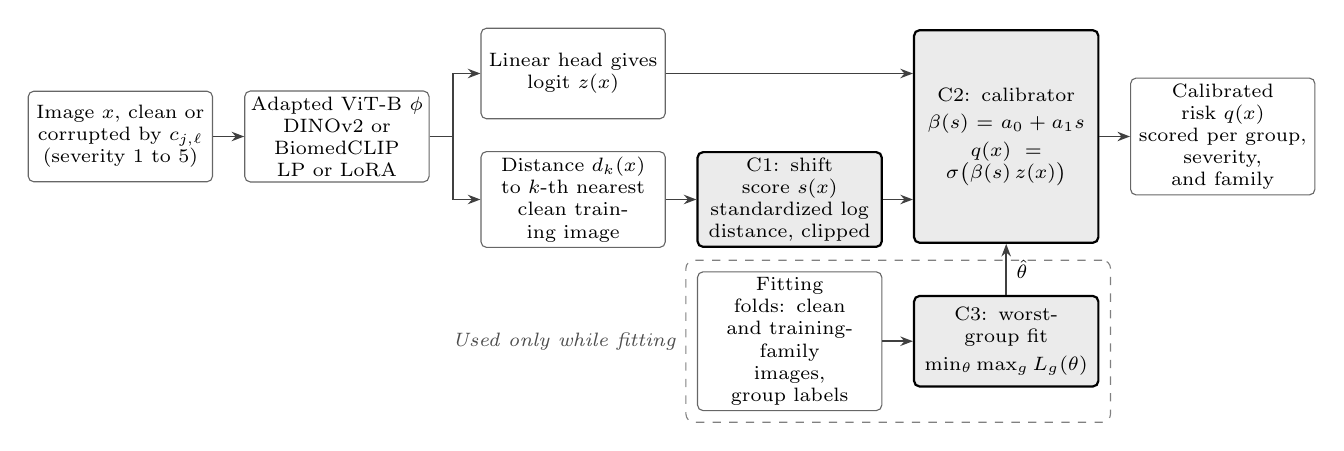
\begin{tikzpicture}[
      font=\scriptsize,
      blk/.style={draw=black!60, rounded corners=2pt, align=center,
        text width=2.2cm, minimum height=1.15cm, inner sep=2pt},
      mine/.style={blk, fill=black!8, draw=black, thick},
      arr/.style={-{Stealth[length=1.6mm]}, semithick, draw=black!75}]
    \node[blk] (input) at (0,0) {Image $x$, clean or\\corrupted by $c_{j,\ell}$\\(severity 1 to 5)};
    \node[blk] (enc) at (2.75,0) {Adapted ViT-B $\phi$\\DINOv2 or BiomedCLIP\\LP or LoRA};
    \node[blk] (logit) at (5.75,0.8) {Linear head gives\\logit $z(x)$};
    \node[blk] (knn) at (5.75,-0.8) {Distance $d_k(x)$\\to $k$-th nearest\\clean training image};
    \node[mine] (score) at (8.5,-0.8) {C1: shift score $s(x)$\\standardized log\\distance, clipped};
    \node[mine, minimum height=2.7cm] (cal) at (11.25,0) {C2: calibrator\\[2pt]$\beta(s) = a_0 + a_1 s$\\[2pt]$q(x) = \sigma\big(\beta(s)\, z(x)\big)$};
    \node[blk] (risk) at (14.0,0) {Calibrated risk $q(x)$\\scored per group,\\severity, and family};
    \node[blk] (fitdata) at (8.5,-2.6) {Fitting folds: clean\\and training-family\\images, group labels};
    \node[mine] (obj) at (11.25,-2.6) {C3: worst-group fit\\[2pt]$\min_{\theta}\max_{g} L_g(\theta)$};
    \node[draw=black!50, dashed, rounded corners=3pt, inner sep=4pt, fit=(fitdata)(obj),
      label={[font=\scriptsize\itshape, text=black!70]left:Used only while fitting}] {};
    \draw[arr] (input) -- (enc);
    \draw[arr] (enc.east) -- ++(0.3,0) |- (logit.west);
    \draw[arr] (enc.east) -- ++(0.3,0) |- (knn.west);
    \draw[arr] (logit.east) -- (logit.east -| cal.west);
    \draw[arr] (knn) -- (score);
    \draw[arr] (score.east) -- (score.east -| cal.west);
    \draw[arr] (cal) -- (risk);
    \draw[arr] (fitdata) -- (obj);
    \draw[arr] (obj) -- node[right] {$\hat{\theta}$} (cal);
  \end{tikzpicture}
  \caption{Overview of the proposed methodology. Shaded blocks are the proposed components of Section~\ref{sec:components}. Group labels are used only in the dashed fitting step, so at test time the calibrator needs only the image and the adapted model.}
  \Description{A flow diagram. An image, clean or corrupted, goes into an adapted ViT-B backbone. The backbone feeds a linear head that gives a logit, and a nearest-neighbor distance to clean training images. The distance becomes a standardized shift score. The logit and the shift score go into the calibrator, which computes an inverse temperature from the score and rescales the logit to give a calibrated risk that is scored per group and severity. Below, inside a dashed box labeled used only while fitting, fitting folds with group labels feed a worst-group fit that sends the fitted parameters up to the calibrator.}
  \label{fig:framework}
\end{figure*}

GR-SATS is a post-hoc calibrator. Its input is an adapted model's logit and feature vector for one image, and its output is a calibrated probability that the lesion is malignant. It has three components. A shift score (C1) measures how far the image's features are from clean training features, a calibrator (C2) turns that score into an inverse temperature that rescales the logit, and a worst-group fit (C3) picks the calibrator's two parameters using group labels on the fitting data. A fourth component (C4) is the literal version of the approved idea, DAC fit for the worst group, which I use to separate the effect of the objective from the effect of the parameterization.

\subsection{Problem Formulation}
\label{sec:formulation}

Each example is an image $x$ with a label $y \in \{0,1\}$, where $y = 1$ means malignant. Let $\mathcal{G}$ be a set of patient groups. For Fitzpatrick17k, $\mathcal{G}$ holds the skin-type groups I-II, III-IV, and V-VI. For HAM10000 it holds four overlapping groups (female, male, under 60, and 60 or older), so each image is in one sex group and one age group. An adapted model $f = h \circ \phi$ has a backbone $\phi$, which maps an image to a feature vector $v(x)$, and a linear head $h$, which gives a logit $z(x)$ and an uncalibrated probability $\sigma(z(x))$, where $\sigma$ is the sigmoid. A corruption $c_{j,\ell}$ applies corruption type $j$ at severity $\ell \in \{1, \dots, 5\}$, and $\ell = 0$ means clean. Each corruption type belongs to one of five families.

A post-hoc calibrator $q_\theta$ maps $z(x)$ and $v(x)$ to a calibrated probability $q_\theta(x)$. It never sees $y$ or the group at test time. It is fit on a set $D$ of clean and corrupted images with labels and group labels, using only some of the corruption families, and it is tested on images corrupted by a family that was left out. The goal is calibration within every group under this kind of shift,
\begin{equation}
  \Pr\big(Y = 1 \mid q_\theta(X) = p,\ X \in g\big) \approx p,
  \label{eq:goal}
\end{equation}
for every probability $p \in [0,1]$ and every group $g \in \mathcal{G}$. Equation~\eqref{eq:goal} cannot be checked directly with small groups, so I measure it with each group's NLL and Brier score and focus on the worst group.

\subsection{Overall Framework}

Figure~\ref{fig:framework} shows the pipeline. An image, either clean or corrupted with one of the MedMNIST-C corruptions, goes through the adapted backbone. The head gives the logit $z$, and the feature $v$ is compared with a bank of clean training features to get the distance $d_k$ to its $k$-th nearest neighbor. The shift score $s$ standardizes and clips that distance (C1). The calibrator turns $s$ into an inverse temperature and rescales the logit (C2). Its two parameters come from the worst-group fit (C3), which is the only step that uses group labels and is done once on the fitting folds. At test time the calibrator needs only the image, so it can be added to any adapted model. The output is a calibrated probability of malignancy, which is scored for every group and severity on corruption families that the fit did not use.

\subsection{Proposed Components}
\label{sec:components}

\textbf{C1. Standardized shift score.} Following DAC \cite{tomani2023dac}, the score starts from a $k$-nearest-neighbor ($k$-NN) distance, the Euclidean distance $d_k(x)$ between the L2-normalized feature $v(x)$ and its $k$-th nearest neighbor in a bank of normalized features of the clean training images. Unlike DAC, I use a single layer, the feature the head receives, and I standardize the log distance,
\begin{equation}
  s(x) = \operatorname{clip}\left(\frac{\log d_k(x) - m}{r},\ s_{\min},\ s_{\max}\right),
  \label{eq:score}
\end{equation}
where $m$ and $r$ are the mean and standard deviation of $\log d_k$ over the clean fitting images and $[s_{\min}, s_{\max}]$ is the range of scores seen during fitting. The input is one image's feature and the output is one number, computed without labels or groups. The log makes the skewed distances more symmetric, and the standardization makes the score unitless, so the same calibrator works for both backbones and both adaptation strategies. I standardize with clean fitting images and not with distances among training images, because fine-tuned models pull training features closer together than features of new images. A percentile of clean distances would also be unitless, but it saturates once corruption pushes an image past every clean image. The clipping keeps a new corruption from pushing the temperature outside the fitted range. Because the bank comes from the training split, a corrupted image is never matched with its own clean copy, and no held-out images are used up. This component addresses Challenge 2.

\textbf{C2. Shift-dependent inverse temperature.} The calibrated probability is
\begin{equation}
  q_\theta(x) = \sigma\big(\beta_\theta(s(x))\, z(x)\big), \qquad \beta_\theta(s) = a_0 + a_1 s,
  \label{eq:calib}
\end{equation}
with $\theta = (a_0, a_1)$ in the set $\Theta$ where $\beta_\theta(s_{\min}) \geq \epsilon$ and $\beta_\theta(s_{\max}) \geq \epsilon$. Its input is the logit and the shift score of one image, and its output is the calibrated probability. Since $\beta_\theta$ is linear, these two constraints keep it positive on the whole clipped range, so the calibrated logit keeps the sign of $z$ and the predicted class at the 0.5 threshold never changes. With $a_1 = 0$ this is ordinary TS with temperature $1/a_0$, which is also a useful check on the code. DAC instead makes the temperature itself a linear function of distances from many layers and fits it with a squared error. Putting the linear model on the inverse temperature is what makes the worst-group fit convex, which is how this component serves Challenge 1. A temperature can only make predictions more or less confident, so it cannot fix a group whose risks are too high or too low across the board, and the base-rate gaps in Section~\ref{sec:data} make that likely. I therefore also test a bias variant, $q_\theta(x) = \sigma(\beta_\theta(s)\, z + b_0 + b_1 s)$, with four parameters. Its fit is still convex, but it can move an image across the 0.5 threshold, so I report accuracy and the area under the ROC curve (AUC) for it and pick the main version at the go/no-go point (Section~\ref{sec:gonogo}).

\textbf{C3. Worst-group objective.} Let $D_{g,\ell}$ be the fitting images of group $g$ at severity $\ell$, where $\ell = 0$ is clean and severities 1 to 5 use only the training corruption families. The loss of group $g$ is
\begin{equation}
  L_g(\theta) = \frac{1}{6}\sum_{\ell=0}^{5}\frac{1}{|D_{g,\ell}|}\sum_{(x,y)\in D_{g,\ell}} -\log q_\theta(y \mid x),
  \label{eq:grouploss}
\end{equation}
with $q_\theta(1 \mid x) = q_\theta(x)$ and $q_\theta(0 \mid x) = 1 - q_\theta(x)$. Like GroupDRO \cite{sagawa2020groupdro}, the fit minimizes the loss of the worst group,
\begin{equation}
  \hat{\theta} = \arg\min_{\theta \in \Theta}\ \max_{g \in \mathcal{G}}\ L_g(\theta).
  \label{eq:objective}
\end{equation}
The input is the logits, shift scores, labels, and group labels of the fitting images, and the output is $\hat{\theta}$. Each $L_g$ averages logistic losses of $\beta_\theta(s)\, z$, which is linear in $\theta$, so $L_g$ is convex, the maximum over groups is convex, and $\Theta$ is set by linear constraints. So every local optimum of Eq.~\eqref{eq:objective} is global, and I solve it exactly in epigraph form by minimizing $t$ subject to $L_g(\theta) \leq t$ for every group. The factor $1/6$ gives clean images and each severity the same weight. Without it, the 55 to 65 corrupted copies of each image from the training families would swamp the clean image. Raw NLL also reflects how hard a group is to classify, so the fit could chase a group that is hard but already calibrated. A second version therefore minimizes the excess loss $L_g(\theta) - \min_{\theta' \in \Theta} L_g(\theta')$, which keeps the focus on miscalibration. This component addresses Challenge 1, and it is what separates GR-SATS from DAC and AAR, which are both fit for average calibration.

\textbf{C4. DAC fit for the worst group.} The approved idea was to change DAC so that it targets the worst group. GR-SATS is a simplified version of that, so I also test the literal version, which I call DAC-WG. It keeps DAC's calibrated probability $\sigma(z(x)/S_w(x))$ with temperature $S_w(x) = w_0 + \sum_l w_l\, d_k^{(l)}(x)$, a weighted sum of $k$-NN distances over the layers DAC uses for ViT-Base with nonnegative weights, and fits it with the worst-group objective of Eq.~\eqref{eq:objective} in place of DAC's average squared error. This loss is not convex in $w$, so I use GroupDRO's alternating updates, with gradient steps on $w$ and exponentiated-gradient steps on the group weights \cite{sagawa2020groupdro}. Comparing DAC with DAC-WG isolates the objective, and comparing DAC-WG with GR-SATS isolates the parameterization.

\textbf{Why this design.} I kept the calibrator to two parameters on purpose. The worst group in Fitzpatrick17k has a few dozen cancers even after pooling, so anything more flexible would overfit it, and two parameters are easy to inspect. Retraining methods such as GroupDRO or Cluster-Focal would need a new model for every attribute and adaptation strategy, while a post-hoc calibrator runs on saved outputs in seconds. Group-wise TS needs group labels at test time, which are often missing or sensitive, so I only use it as a reference. Table~\ref{tab:mapping} maps each challenge to the components.

\begin{table}[t]
  \caption{Mapping between research challenges and proposed methods.}
  \label{tab:mapping}
  \scriptsize
  \setlength{\tabcolsep}{3pt}
  \renewcommand{\arraystretch}{1.1}
  \begin{tabularx}{\columnwidth}{@{}P{1.3cm}LLL@{}}
    \toprule
    \textbf{Challenge} & \textbf{Technique} & \textbf{Function} & \textbf{Expected effect} \\
    \midrule
    1. Worst-off group under shift & Worst-group fit (C3) of an inverse temperature that is linear in the shift score (C2), with an excess-NLL variant & Picks the two parameters that minimize the largest group loss, as a convex problem & Lower worst-group NLL and Brier score under corruption, with the cost to other groups visible \\
    \addlinespace
    2. Shift signal that transfers & Standardized, clipped log $k$-NN distance (C1) and leave-one-family-out testing & Gives a unitless score that grows with severity and stays in the fitted range & Calibration that holds on unseen corruption families, for both LP and LoRA \\
    \addlinespace
    3. Small groups & Cross-fitting over the pooled splits, proper scores, paired bootstrap over source images, fixed primary comparisons & Uses every pooled image for testing and gives honest uncertainty & Conclusions about groups with a few dozen cancers that are not driven by noise \\
    \bottomrule
  \end{tabularx}
\end{table}

%% =========================================================
\section{Experimental Methodology}
\label{sec:experiments}

\subsection{Dataset}
\label{sec:data}

I use two public dermatology datasets that have binary malignancy labels and patient group labels.

HAM10000 \cite{tschandl2018ham10000} has 10,015 dermoscopic images of 7,470 pigmented lesions in seven diagnostic categories, with the patient's sex and age, and I take the images from the Harvard Dataverse.\footnote{\url{https://doi.org/10.7910/DVN/DBW86T}} I use the DermaMNIST-C splits of Abhishek et al.\ \cite{abhishek2025quality}, who moved every image of a training lesion out of the validation and test splits, so no lesion crosses splits. The label is malignant for melanoma, basal cell carcinoma, and actinic keratosis or intraepithelial carcinoma, and benign otherwise. MEDFAIR counts basal cell carcinoma as benign \cite{zong2023medfair}, but it is a skin cancer, so I keep the clinical definition. The groups are sex and age, with age split at 60 as in MEDFAIR.

Fitzpatrick17k \cite{groh2021fitzpatrick} has 16,577 clinical photos of 114 skin conditions with Fitzpatrick skin type labels. I use the cleaned Fitzpatrick17k-C \cite{abhishek2025quality}, which removes duplicates and leaves 11,394 images with fixed training, validation, and test splits, and I match its label file\footnote{\url{https://doi.org/10.5281/zenodo.11101337}} to Abhishek et al.'s image archive by file hash. The label is malignant versus everything else, meaning benign and non-neoplastic cases together, which is the same binary label MEDFAIR uses for this dataset. Limiting the task to benign versus malignant would drop most of the images and leave too few cancers in the darkest skin types. I merge the six skin types into I-II, III-IV, and V-VI so that each group has enough cases.

Following MEDFAIR, I drop images whose group attribute was not recorded, which removes 67 HAM10000 images and 296 Fitzpatrick17k-C images. HAM10000 is left with 9,948 images of 7,414 lesions, the same image count MEDFAIR and FairMedFM use \cite{zong2023medfair,jin2024fairmedfm}. Table~\ref{tab:data} gives the counts. Two features of the data matter for calibration. In HAM10000, lesions with several photos ended up almost entirely in the training split (1,876 of 1,956), and their photos are more often malignant (31\% versus 10\% for single-photo lesions), so 21.3\% of training images are malignant compared with 11.9\% of the pooled validation and test images. In Fitzpatrick17k-C, 8.8\% of the pooled V-VI images are malignant compared with 16.0\% of the I-II images. A temperature alone cannot correct risks that are off in one direction, which is why I also test the bias variant of C2.

For shift I use the 15 dermatology corruptions of MedMNIST-C \cite{disalvo2024medmnistc}, each at five severities, through its public library.\footnote{\url{https://github.com/francescodisalvo05/medmnistc-api}} They fall into five families, digital (JPEG and pixelate), noise (Gaussian, speckle, impulse, and shot), blur (defocus, motion, and zoom), color (brightness and contrast, each up and down), and task-specific (black corners and text overlays). The task-specific family imitates dermoscope artifacts, so it is less realistic for Fitzpatrick17k's clinical photos, and I report it separately there. Both datasets are public, have the group labels I need, and are small enough to run the whole grid on free Colab GPUs. CheXpert \cite{irvin2019chexpert}, with sex, age, and race, is planned as an extension after the semester.

\begin{table}[t]
  \caption{Data after removing images with an unrecorded group attribute. Each cell gives images, with malignant cases in parentheses. The pool is the validation and test splits together, which the calibrators use through 5-fold cross-fitting.}
  \label{tab:data}
  \footnotesize
  \begin{tabular}{@{}lrr@{}}
    \toprule
     & \textbf{HAM10000} & \textbf{Fitzpatrick17k-C} \\
    \midrule
    Training split & 8,164 (1,740) & 7,779 (1,144) \\
    Validation split & 568 (63) & 1,100 (154) \\
    Test split & 1,216 (149) & 2,219 (325) \\
    Pool & 1,784 (212) & 3,319 (479) \\
    Malignant, training & 21.3\% & 14.7\% \\
    Malignant, pool & 11.9\% & 14.4\% \\
    \midrule
    \multicolumn{3}{@{}l}{\textit{Groups in the pool}} \\
    Female & 820 (80) & \\
    Male & 964 (132) & \\
    Age under 60 & 1,206 (62) & \\
    Age 60 or older & 578 (150) & \\
    Skin type I-II & & 1,794 (287) \\
    Skin type III-IV & & 1,163 (160) \\
    Skin type V-VI & & 362 (32) \\
    \bottomrule
  \end{tabular}
\end{table}

\subsection{Data Preprocessing}

Every image is resized so that its shorter side is 224 pixels and then center-cropped to 224 by 224, the resolution MedMNIST-C's corruption settings were designed for \cite{disalvo2024medmnistc}. Corruptions are applied to this crop, and the result is normalized with each backbone's own mean and standard deviation. Each corrupted image is generated from a seed made of the image, the corruption, and the severity, so every model sees exactly the same corrupted images and the data loader can rebuild them instead of storing about 75 copies of every pooled image, which would take close to 60 GB. Training uses only geometric augmentation, namely random resized crops with scale 0.8 to 1, flips, and 90-degree rotations. I leave out color and blur augmentation on purpose, because they overlap with the test corruptions. I also do not reweight the classes, since reweighting would push predicted probabilities away from the true rates. No missing values remain after the images with unrecorded groups are dropped. Everything learned from data, including the linear probes, the reference bank, the shift-score standardization, AAR's class-conditional Gaussians, the k-means clusters, and every calibrator, uses only the training split or the fitting folds.

\subsection{Data Splitting and Validation}
\label{sec:splits}

Models are trained on the official training split. I hold out 10\% of it, grouped by lesion for HAM10000, as a development slice for early stopping and for choosing the probe's regularization, and the reference bank uses the remaining training images. The validation and test splits are pooled and split into five folds, stratified by group and label (sex, age group, and label for HAM10000), with all images of a lesion and all corrupted copies of an image kept in the same fold. For each fold $f$ and each corruption family $h$, a calibrator is fit on the clean images outside $f$ and on their corrupted copies from the four families other than $h$. It is then applied to the clean images in $f$ and to their copies corrupted with $h$. So every pooled image is tested once for each family, by a calibrator that never saw that image or that family. Compared with fitting on the validation split alone, each fit sees more than twice as many images, and the final metrics use the whole pool, which for skin types V and VI is 362 images and 32 cancers. Every model is trained with three seeds. This protocol uses the small groups as fully as possible, avoids leakage between lesions, and tests generalization to corruptions that were not available when the calibrator was fit.

\subsection{Baseline Methods}
\label{sec:baselines}

\begin{itemize}
  \item \textbf{Baseline 1, simple global calibrators.} This group has no calibration, TS fit on the clean fitting images \cite{guo2017calibration}, TS fit on fitting images perturbed with Gaussian noise as in Tomani et al.\ \cite{tomani2021posthoc}, TS fit on the clean images plus my training corruption families, and TS with exposure to unrelated texture images labeled 0.5, which Roschewitz et al.\ found most robust under natural shift \cite{roschewitz2025where}. TS with my corruption families is the strongest simple baseline and one of the three primary comparisons.
  \item \textbf{Baseline 2, shift-aware calibrators.} DAC \cite{tomani2023dac} runs with its official code and is fit on the same clean and corrupted images as my method, and I also report its published clean-only fit. Multi-domain TS \cite{yu2022multidomain} fits a temperature for each training corruption and severity and then regresses the temperature on the features. AAR \cite{yuksekgonul2023atypicality} is fit on the same data as my method. DAC is the seed method I build on and AAR is the closest existing method, so both are primary comparisons.
  \item \textbf{Baseline 3, group-aware calibrators.} Cluster-wise TS in the style of FairCal \cite{salvador2022faircal} runs k-means on the fitting features, fits one temperature per cluster, and assigns each test image to its nearest cluster. It is the most direct existing way to target subgroups without test-time labels. I also report group-wise TS, which uses group labels at test time but does not adapt to shift, and a per-group version of GR-SATS that uses both, as an oracle.
\end{itemize}

\subsection{Implementation Details}

I will write the code in Python with PyTorch. The backbones are DINOv2 ViT-B/14 \cite{oquab2024dinov2}, a self-supervised model distilled from a larger one trained on 142 million curated natural images, and the ViT-B/16 image encoder of BiomedCLIP \cite{zhang2025biomedclip}, a CLIP-style model \cite{radford2021clip} trained on 15 million biomedical figure and caption pairs from PubMed Central. Both are ViT-Base models \cite{dosovitskiy2021vit}, so pretraining is the main thing that differs between them, and both are among the FairMedFM models \cite{jin2024fairmedfm}. For LP, I fit an L2-regularized logistic regression on the frozen embedding with scikit-learn and choose the regularization strength from $\{0.01, 0.1, 1, 10\}$ by development-slice NLL. Since the backbone is frozen, the features of every clean and corrupted image are computed once per backbone and shared by all seeds. For LoRA, I add rank-8 adapters with scaling 16 to the query and value projections of every attention block \cite{hu2022lora}, plus a linear head, and train with AdamW (learning rate $3 \times 10^{-4}$, weight decay 0.01, batch size 64, cosine schedule) for at most 20 epochs, keeping the epoch with the lowest development-slice NLL. The loss is unweighted binary cross-entropy, and the seeds are 0, 1, and 2. Nearest neighbors come from FAISS with $k = 10$, the corruptions from the MedMNIST-C library, and DAC and AAR from their official code.\footnote{\url{https://github.com/futakw/DensityAwareCalibration} and \url{https://github.com/mertyg/beyond-confidence-atypicality}} GR-SATS and its variants are solved as convex programs with CVXPY, with $\epsilon = 0.05$. Cluster-wise TS uses $K = 8$ clusters, and the texture set for TS with OOD exposure is 10\% the size of the clean fitting set, the ratio Roschewitz et al.\ found to work well \cite{roschewitz2025where}. The GPU work runs on free Google Colab, which usually provides an NVIDIA T4 with 16 GB of memory, so training and evaluation use 16-bit mixed precision. Free sessions last at most about 12 hours, disconnect when idle, and do not guarantee a GPU, so every job saves checkpoints and outputs to Google Drive and resumes where it stopped, and Kaggle's free notebooks are the backup. The clean images are resized once and stored on Drive, which takes about 3 GB. Free Colab usually gives only two CPU cores, so generating corruptions is slower than the forward passes, and each corrupted batch is therefore generated once and passed through every model trained on the same dataset. The evaluation pass saves only what the calibrators need, mainly logits and distance and atypicality scores, which comes to tens of megabytes per model, so every calibrator fits on a CPU in seconds to minutes. I estimate the core grid at roughly 10 to 20 hours on a T4, most of it for LoRA training and the corrupted evaluation passes, spread over several sessions.

\subsection{Evaluation Metrics}
\label{sec:metrics}

\textbf{Primary metrics.} The main test pools the held-out corruption families at severities 3 to 5, where calibration is most likely to fail. For Fitzpatrick17k the task-specific family is left out of this pool and reported on its own. On the pool I report worst-group NLL and worst-group Brier score, where the worst group is the group with the highest value of that metric for that method. For HAM10000 the worst group is taken over all four sex and age groups, and I also report each attribute separately. Both metrics are proper scoring rules \cite{brier1950verification,gruber2022proper}, so a method cannot improve them by reporting anything other than its best estimate of the true probability, and both are much less noisy than binned ECE for groups of a few hundred images.

\textbf{Secondary metrics.} I report NLL and Brier score for every group, which shows whether a method narrows the gap by making the better-off groups worse \cite{zong2023medfair}, plus the average NLL over all images, which shows what the worst-group fit costs. ECE is computed with 15 equal-mass bins, which Roelofs et al.\ found less biased than equal-width bins \cite{roelofs2022mitigating}, alongside the debiased estimator of the squared calibration error from Kumar et al.\ \cite{kumar2019verified}. I also report the ECE gap between groups, the area under the curve of ECE against severity, AUC, and accuracy for the methods that can change predictions. AUC matters because a per-image temperature can reorder images even though it keeps every predicted class. Accuracy alone would be misleading, since only 12\% of the pooled HAM10000 images and 14\% of the pooled Fitzpatrick17k-C images are malignant. On clean images I report ECE and AUC to measure the in-distribution cost that Roschewitz et al.\ warn about \cite{roschewitz2025where}.

\textbf{Statistics.} I fix three primary comparisons in advance, GR-SATS against TS fit with my corruption families, against DAC, and against AAR. For each one, success means a lower worst-group NLL and Brier score averaged over the 8 core settings, with a 95\% paired bootstrap interval that excludes zero. The bootstrap resamples source images 2,000 times (lesions for HAM10000) instead of corrupted copies, since the copies of one image are not independent. Metrics are averaged over the three seeds before the comparison. I also expect GR-SATS to close at least half of the worst-group NLL gap between TS with corruptions and the per-group oracle, and on clean images to stay within 0.01 ECE and 1 AUC point of clean TS. I will report per-setting results too, but to rank all methods across settings without dozens of pairwise tests, I use the Friedman test with the Nemenyi post-hoc test, as MEDFAIR does \cite{zong2023medfair}.

%% =========================================================
\section{Results and Analysis}
\label{sec:results}

No experiments have been run yet, so this section sets up the tables and analyses that the final paper will fill in. Every entry is to be determined (TBD).

\subsection{Main Results}

\begin{table}[t]
  \caption{Planned main results on unseen corruption families at severities 3 to 5, averaged over the 8 core settings. WG means worst group, and $\dagger$ marks methods that use group labels at test time.}
  \label{tab:results}
  \scriptsize
  \setlength{\tabcolsep}{3.5pt}
  \begin{tabular}{@{}lccccc@{}}
    \toprule
    \textbf{Method} & \textbf{WG NLL} & \textbf{WG Brier} & \textbf{NLL} & \textbf{Clean ECE} & \textbf{AUC} \\
    \midrule
    No calibration & TBD & TBD & TBD & TBD & TBD \\
    TS, clean & TBD & TBD & TBD & TBD & TBD \\
    TS with Gaussian noise & TBD & TBD & TBD & TBD & TBD \\
    TS with corruptions & TBD & TBD & TBD & TBD & TBD \\
    TS with textures & TBD & TBD & TBD & TBD & TBD \\
    DAC & TBD & TBD & TBD & TBD & TBD \\
    Multi-domain TS & TBD & TBD & TBD & TBD & TBD \\
    AAR & TBD & TBD & TBD & TBD & TBD \\
    Cluster-wise TS & TBD & TBD & TBD & TBD & TBD \\
    GR-SATS (proposed) & TBD & TBD & TBD & TBD & TBD \\
    \midrule
    Group-wise TS$^\dagger$ & TBD & TBD & TBD & TBD & TBD \\
    Per-group GR-SATS$^\dagger$ & TBD & TBD & TBD & TBD & TBD \\
    \bottomrule
  \end{tabular}
\end{table}

Table~\ref{tab:results} will report the primary and secondary metrics of every method, averaged over the 8 core settings, with per-setting tables in an appendix. I will test three hypotheses. \textbf{H1.} The worst-group NLL of clean-fit TS rises with severity, and it rises faster for the worst group than for the best one. \textbf{H2.} The severity at which clean-fit TS starts doing harm, meaning a higher worst-group NLL than no calibration at all, differs between LP and LoRA. \textbf{H3.} GR-SATS meets the success criteria of Section~\ref{sec:metrics} against all three primary comparisons. H1 and H2 are measurements, so they are worth reporting whatever happens with H3.

\subsection{Ablation Study}

\begin{table}[t]
  \caption{Planned ablation on the same test pool. The first four rows cross a global or shift-aware temperature with an average or worst-group loss.}
  \label{tab:ablation}
  \scriptsize
  \begin{tabular}{@{}llcc@{}}
    \toprule
    \textbf{Temperature} & \textbf{Loss} & \textbf{WG NLL} & \textbf{NLL} \\
    \midrule
    Global & Average (TS with corruptions) & TBD & TBD \\
    Global & Worst group & TBD & TBD \\
    Shift-aware & Average & TBD & TBD \\
    Shift-aware & Worst group (GR-SATS) & TBD & TBD \\
    \midrule
    \multicolumn{2}{@{}l}{GR-SATS with excess NLL} & TBD & TBD \\
    \multicolumn{2}{@{}l}{GR-SATS with bias term} & TBD & TBD \\
    \multicolumn{2}{@{}l}{DAC, average loss} & TBD & TBD \\
    \multicolumn{2}{@{}l}{DAC-WG, worst-group loss} & TBD & TBD \\
    \multicolumn{2}{@{}l}{AAR, average loss} & TBD & TBD \\
    \multicolumn{2}{@{}l}{AAR-WG, worst-group loss} & TBD & TBD \\
    \bottomrule
  \end{tabular}
\end{table}

Table~\ref{tab:ablation} crosses a global or shift-aware temperature with an average or worst-group loss. The global temperature with average loss is TS fit with my corruption families, the kind of simple baseline Roschewitz et al.\ found hard to beat \cite{roschewitz2025where}. If the shift-aware, worst-group cell beats both cells that change only one part, then both parts matter. The lower half of the table applies the worst-group loss to DAC's and AAR's parameterizations as well. If the worst-group version wins for all three parameterizations, the gain comes from the objective and not from my shift score. I will also report the excess-NLL and bias variants and a sensitivity check over $k \in \{1, 10, 50\}$.

\subsection{Error and Failure Analysis}
\label{sec:failure}

Per-group reliability diagrams at each severity will show whether the errors come from overconfidence, which a temperature can fix, or from risks that are off in one direction, which needs the bias variant. Per-family results will show which corruptions break the calibrator, for example whether changes in brightness and contrast hurt darker skin types more. To separate the two reasons a group's shift scores can be high, I will check whether the gap in shift scores between groups grows with severity beyond its clean value, and rerun the method with a reference bank that has the same number of images from each group. Whether the method helps the worst group does not depend on which reason is behind it, so the method itself is judged with the standard bank. I will also check how the HAM10000 base-rate gap between training and evaluation shows up in the reliability diagrams, and whether the worst group changes between LP and LoRA.

%% =========================================================
\section{Project Execution Plan}
\label{sec:plan}

\subsection{Six-Week Research and Implementation Plan}

Table~\ref{tab:plan} lists the weekly objectives, tasks, and milestones from October 19 to November 29, 2026. The plan moves from the data pipeline and a pilot in the first two weeks, to the method and baselines in Week 3, the main experiments in Week 4, the ablation and failure analysis in Week 5, and the final paper in Week 6.

\begin{table*}[t]
  \caption{Six-week research and implementation plan.}
  \label{tab:plan}
  \scriptsize
  \setlength{\tabcolsep}{4pt}
  \renewcommand{\arraystretch}{1.15}
  \begin{tabularx}{\textwidth}{@{}P{1.3cm}P{2.1cm}LP{4.6cm}P{1.15cm}@{}}
    \toprule
    \textbf{Week} & \textbf{Objective} & \textbf{Specific tasks} & \textbf{Expected output or milestone} & \textbf{Member} \\
    \midrule
    1 (Oct 19 to 25) & Data pipeline and linear probes & Write loaders for HAM10000 and Fitzpatrick17k-C with the label and group rules of Section~\ref{sec:data}, and store the resized images on Google Drive. Set up Colab notebooks that checkpoint to Drive and resume after a disconnect. Build the five cross-fitting folds and the development slice. Set up the 15 MedMNIST-C corruptions at 224 pixels with per-image seeds. Extract frozen DINOv2 and BiomedCLIP features and train linear probes with three seeds. & Counts that match Table~\ref{tab:data}, a check that no lesion crosses folds, a Colab job that resumes correctly after a forced disconnect, a grid of every corruption at every severity, and clean AUC for all 12 linear probes. & Adit Patel \\
    \addlinespace
    2 (Oct 26 to Nov 1) & LoRA models and pilot & Train the 12 LoRA models (2 datasets, 2 backbones, 3 seeds). Run the evaluation pass that saves logits, distances, and atypicality scores for all clean and corrupted pooled images. Fit clean TS, run the headroom check, plot per-group NLL and ECE against severity, and test whether shift scores differ between groups. & Pilot report with per-group severity curves and reliability diagrams, and a written go/no-go decision with the choice of main variant by November 1. & Adit Patel \\
    \addlinespace
    3 (Nov 2 to 8) & Method and baselines & Implement GR-SATS with its excess-NLL and bias variants, and DAC-WG. Implement the baselines of Section~\ref{sec:baselines} using the official DAC and AAR code. Build the cross-fitting and leave-one-family-out harness, with unit tests for zero slope giving TS, no flipped predictions, and disjoint folds. & Every calibrator runs end to end on one setting, and my TS and DAC numbers match the official code there. & Adit Patel \\
    \addlinespace
    4 (Nov 9 to 15) & Main experiments & Run every calibrator on the 8 core settings with three seeds. Compute all metrics of Section~\ref{sec:metrics}, the paired bootstrap for the three primary comparisons, and the Friedman and Nemenyi tests. & Filled Table~\ref{tab:results}, per-severity curves, bootstrap intervals, and a verdict on H1 to H3. & Adit Patel \\
    \addlinespace
    5 (Nov 16 to 22) & Ablation and failure analysis & Fill Table~\ref{tab:ablation}, including DAC-WG, AAR-WG, and the sensitivity check over $k$. Run the analyses of Section~\ref{sec:failure}, including the group-balanced bank and the separate task-specific family for Fitzpatrick17k. Start the ImageNet ViT if ahead of schedule. & Ablation table, reliability diagrams, per-family results, and a written analysis of why the method helps or fails. & Adit Patel \\
    \addlinespace
    6 (Nov 23 to 29) & Final results and reproducibility & Run the stretch goals if time allows. Rerun one setting from scratch to confirm the numbers. Write the results, discussion, and limitations, and update the abstract with real numbers. Prepare the final presentation. & Final paper with all tables and figures, plus code and scripts that rebuild every table. & Adit Patel \\
    \bottomrule
  \end{tabularx}
\end{table*}

\subsection{Go/No-Go Decision and Scope}
\label{sec:gonogo}

The end of Week 2 is the go/no-go point. Liu et al.\ showed that ordinary training often gives group calibration on its own \cite{liu2019implicit}, so I first check that there is something to fix. The pilot passes if, on at least one dataset, two things hold. First, fitting the two-parameter calibrator directly on the evaluation images with the worst-group loss has to lower worst-group NLL by more than one bootstrap standard error compared with the average loss. If it barely helps even there, it cannot help on unseen corruptions. Second, the worst group's mean shift score has to differ from the other groups' at severities 3 to 5, with a bootstrap interval that excludes zero, or a group-blind calibrator has nothing to work with. If neither dataset passes both checks, I will switch to the measurement study, which reports the severity at which clean-fit calibration starts doing harm under each adaptation strategy and whether one calibrator transfers across strategies. The per-group reliability diagrams from the pilot also decide whether the temperature-only or the bias version of C2 is the main one.

The core result I am committing to this semester is the 8 core settings with three seeds. If that finishes early, I will add an ImageNet-supervised ViT-B/16 \cite{dosovitskiy2021vit} first and full fine-tuning second. CheXpert \cite{irvin2019chexpert}, an LVM-Med ResNet-50 against an ImageNet ResNet-50 \cite{nguyen2023lvmmed,he2016resnet}, and CLIP-Adapt for BiomedCLIP would come after the semester. If compute runs short, I will cut the seeds from three to two before cutting any settings.

\subsection{Changes Since the Approved Proposal}

A few things changed after the project was approved. The title now names the method, since the method is more specific than when I proposed it. The core grid is 2 backbones by 2 adaptation strategies, and the ImageNet-supervised ViT and full fine-tuning are now stretch goals, because I had no experiment code in early October and would rather finish a smaller grid well. I wrote my own loaders for the skin datasets instead of using the FairMedFM code, because HAM10000 needs lesion-level splits and I count basal cell carcinoma as malignant, while MEDFAIR splits images at random by default and counts basal cell carcinoma as benign \cite{zong2023medfair}. FairMedFM also does not include Fitzpatrick17k. The pilot moved from mid-October to a go/no-go decision by November 1. During the survey I found AAR \cite{yuksekgonul2023atypicality}, the closest existing method, so it is now a main baseline, and I added DAC-WG so that the exact idea that was approved, DAC changed to target the worst group, is tested directly. Finally, the statistics plan in Section~\ref{sec:metrics} is new, since I left it out of the short proposal.

%% =========================================================
\section{Team Member Contributions}

I am the only member of this team, so every task in Table~\ref{tab:plan} is mine. So far I chose the topic, wrote the project plan and revised it after feedback, set the scope and selection criteria of the survey, built the Connected Papers graphs for both seeds, downloaded the datasets, and reviewed the paper list and the text. For the rest of the semester I am responsible for the data pipeline and corruption code, training the linear probes and LoRA models, implementing GR-SATS and the baselines, running the experiments and statistical tests, making the figures, and writing the final paper. An LLM assistant helps with parts of this work, as described in Section~\ref{sec:llm}.

%% =========================================================
\section{Use of Generative AI and LLM Tools}
\label{sec:llm}

I used Claude Opus 5.5 (Anthropic) through the Claude Code agent in every phase. In Phase 0 it helped me set up the ACM LaTeX template, edit the wording of my abstract and project proposal, and write a script that downloads the reference PDFs. In Phase 1 it pulled citation lists from the Semantic Scholar Graph API, screened about 450 titles against my criteria, confirmed each kept paper's title, venue, and year, proposed the taxonomy, and drafted the survey text, LaTeX, and BibTeX. It could not use web apps such as Connected Papers, so I built those graphs myself, and the agent compared their paper lists with my collection.

For Phase 2 the agent reorganized the paper to follow the course template and drafted most of the new sections from my detailed project plan, including the equations, the diagram in Figure~\ref{fig:framework}, and the tables. It computed the counts in Table~\ref{tab:data} with a short Python script that reads the DermaMNIST-C and Fitzpatrick17k-C label files, and it checked each new statement about another paper against that paper's PDF instead of relying on the model's memory. No references were added in this phase, so the reference list, the PDF folder, and \texttt{literature\_list.csv} still hold the same 82 papers. During the experiments I plan to use the agent for help with code. Every number in the final paper will come from my own runs, and I will check the code with small tests, for example that GR-SATS reduces to ordinary TS when its slope is zero, that no lesion appears in two folds, and that my TS and DAC results match the official code on one setting. I reviewed and edited the text, and I am responsible for the final content.

%% =========================================================
\section{Conclusion}

This proposal targets a gap between two lines of work. Shift-aware calibrators keep average calibration under corruption, and group-aware calibrators protect groups only when test data look like calibration data. GR-SATS combines the two with a convex, two-parameter, worst-group fit on a standardized shift score. I will test it on HAM10000 and Fitzpatrick17k with DINOv2 and BiomedCLIP adapted by linear probing and LoRA, on corruption families held out from fitting, against strong simple baselines, DAC, and AAR, with worst-group NLL and Brier score as the main metrics and a protocol built for small groups. If the method works, it gives a cheap way to keep risk estimates calibrated for the worst-off patients when image quality drops. If it does not, the study will still show at what corruption level clean-fit calibration stops being safe for each group and adaptation strategy.

\bibliographystyle{ACM-Reference-Format}
\bibliography{references}

\end{document}
